
%% optional, but if you want to list author:

\introauthor{Rolly Maulana Awangga, S.T., M.T.}
{Informatics Research Center\\
Bandung, Jawa Barat, Indonesia}
Pada era disruptif  \index{disruptif}\index{disruptif!modern} 
saat ini. git merupakan sebuah kebutuhan dalam sebuah organisasi pengembangan perangkat lunak.
Buku ini diharapkan bisa menjadi penghantar para programmer, analis, IT Operation dan Project Manajer.
Dalam melakukan implementasi git pada diri dan organisasinya.

Rumusnya cuman sebagai contoh aja biar keren\cite{awangga2018sampeu}.
\begin{equation}
ABC {\cal DEF} \alpha\beta\Gamma\Delta\sum^{abc}_{def}
\end{equation}

Langkah cepat \textit{create pull request} bagi yang sudah tahap menuju dewasa.
\lstinputlisting[caption=Langkah cepat \textit{create pull request}, label={lst:pullrequest}]{src/pullrequest.tex}

Ingat selalu langkah-langkah seperti pada gambar \ref{fig:langkahawal} dan \ref{fig:createpullrequest}, agar Anda tidak tersesat.
\begin{figure}[!htbp]
\centerline{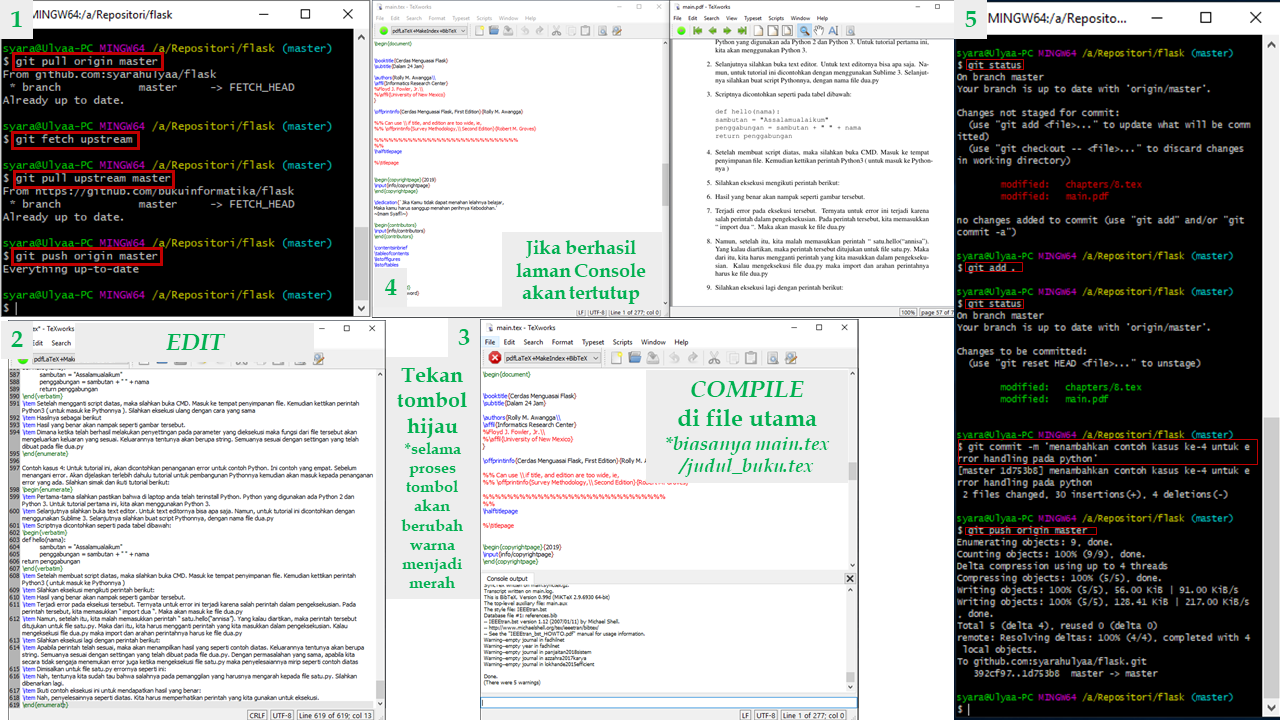
\includegraphics[width=1\textwidth]{Figures/langkahawal.PNG}}
\caption{Langkah awal sebelum \textit{create pull request}}
\label{fig:langkahawal}
\end{figure}

\begin{figure}[!htbp]
\centerline{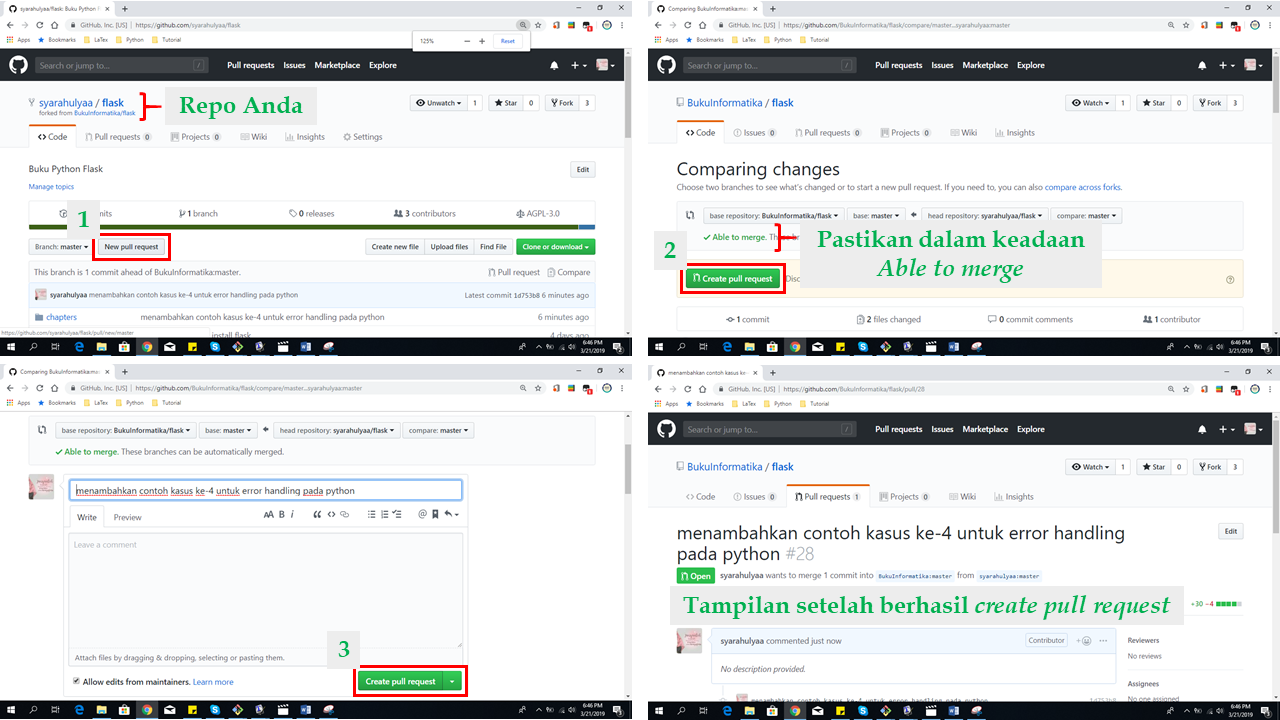
\includegraphics[width=1\textwidth]{Figures/createpullrequest.PNG}}
\caption{Langkah-langkah \textit{create pull request}}
\label{fig:createpullrequest}
\end{figure}